
This chapter focuses on describing the dedicated calibration hardware systems deployed for the \dword{dune} \dword{dp} \dword{fd} module and providing necessary information beyond the reach of external measurements and existing sources and monitors. These include an ionization laser system, a photoelectron laser system, 
and a \dword{pns} system. A possible radioactive source system is also being explored. The responsibility for the calibration hardware systems fall under the joint \dword{sp} and \dword{dp} calibration consortium formed in November 2018.

A detailed understanding of the overall detector response is essential for \dword{dune} physics goals. Each calibration parameter must be measured precisely according to the requirements on the %JM
systematic uncertainties for the \dword{lbl}, low-energy (\dword{snb}), and other physics programs at \dword{dune}. The calibration 
program 
%plan %JM;
must provide stable measurements at a few-percent-or-better 
%few-percent %JM; SG: this was a language edit from editors
level across an enormous volume and over a long period while providing sufficient redundancy. The physics volume of the \dword{tdr} provides a detailed description of the calibration strategy for the \dword{dune} \dword{fd}; here, we provide a brief summary.

The current calibration strategy for \dword{dune} uses existing sources of particles, external measurements, and dedicated external calibration hardware systems. Existing calibration sources for \dword{dune} include beam or atmospheric neutrino-induced samples, cosmic rays, argon isotopes, and instrumentation devices such as \dword{lar} purity and temperature monitors. Dedicated calibration hardware systems comprise laser and neutron source deployment systems.  External measurements by \dword{protodune} and \dword{snb} experiments  will validate techniques, tools, and design of systems for the \dword{dune} calibration program. These sources and systems measure detector response model parameters or provide tests of the response model itself. Calibration measurements can also correct data, data-driven efficiencies, systematics, and particle responses.

%Chapter~4 of the Physics volume of the \dword{tdr} provides a more detailed description of the calibration strategy for the \dword{dune} \dword{fd}. 
%using existing sources of particles (e.g., cosmic ray muons), external measurements (e.g., \dword{protodune}), monitors (e.g., purity monitors), and dedicated calibration hardware systems. 


%This chapter describes the design of the dedicated calibration systems to be deployed for the DUNE \spmod.  As discussed in the Physics TDR\fixme{proper reference}, the calibration strategy includes external measurements (e.g. ProtoDUNE), monitors (e.g. purity, thermal), existing sources of particles (e.g. muons from cosmic rays), and dedicated external calibration hardware systems.  This chapter discusses the calibration hardware systems. Monitoring systems are discussed in other chapters: CISC (purity, thermal monitors, slow control), PDS (LED stability system\fixme{proper name is?}), and CE (charge injection system). The physics TDR discusses the use of existing sources of particles, and external measurements. 

Calibration systems are used at each stage of the experiment. Once the \dword{fd} is filled and at the desired high voltage, it immediately becomes live for 
non-beam physics
%\dword{snb} and proton decay signals (beam and atmospheric neutrino physics will require a few years of data accumulation) 
at which point  %for %JM
early calibration must track %to track %JM
the space-time dependence of the detector. Dedicated early calibration runs using calibration hardware systems develop and tune calibration tools to beam data taking and correct for any space-time irregularities observed in the \dword{tpc}. Given the expected low rate of cosmic ray events at the underground location, calibration using cosmic rays is not possible over short time scales and will proceed from coarse-grained to fine-grained over the course of years, as statistics accumulate. 
The experiment will rely on calibration hardware systems, such as a laser system, for calibrations that require an independent probe with reduced or removed interdependencies, fine-grained measurements (both in space and time), and detector stability monitoring on the time scales required by physics. Calibration systems such as a neutron source system provide low-energy electromagnetic response at the precision required for low-energy \dword{snb} physics. 
Once the detector is running stably, dedicated calibration runs (ideally before, during, and after each run period) will ensure that detector conditions have not changed significantly. As \dword{dune} becomes systematics-limited, dedicated precision-calibration campaigns using the calibration hardware systems must help meet the stringent physics requirements on energy scale reconstruction and detector resolution.

%Section~\ref{sec:sp-calib-ov-scope} describes the baseline calibration hardware designs. 
%and outlines alternative designs that may improve the physics capability and/or reduce overall cost. 
Section~\ref{sec:dp-calib-sys} describes the baseline calibration hardware designs. Section~\ref{sec:dp-calib-sys-las-ion} describes the baseline design for the ionization laser system that provides an independent, fine-grained measurement of the electric field throughout the detector, an essential parameter that affects the spatial and energy resolution of physics signals. The \dword{dune} \dword{cdr}~\cite{Acciarri:2015uup} assumes that the \dword{fv} is known to the \SI{1}{\%} level. By measuring spatial distortions and drift velocity map, the laser calibration system also 
%mainly 
helps define the detector \dword{fv}, thus allowing correct predictions of the \dword{fd} spectra. The laser system also offers many secondary uses such as alignment checks, stability monitoring, and diagnosing detector performance issues. 
%Alternative designs for the ionization laser system that may improve the physics capability and/or reduce overall cost are also under development and are described in Appendix~\ref{sec:sp-calib-laser-alter}.
Section~\ref{sec:dp-calib-sys-las-pe} describes the photoelectron laser system that can be used to rapidly diagnose electronics or \dword{tpc} response issues along with many other useful measurements such as integrated field across drift, drift velocity, and electronics gain. 

Section~\ref{sec:dp-calib-sys-pns} describes the baseline design for the \dword{pns} system, which provides a triggered, well defined energy deposition from neutron capture in Ar detectable throughout the detector volume. Neutron capture is a critical component of signal processes for \dword{snb} and \dword{lbl} physics, enabling direct testing of the detector response spatially and temporally for the low-energy program and the efficiency of the detector in reconstructing the low-energy spectra. The proposed \dword{rsds}, which is in many ways complementary to the \dword{pns} system, can provide at known locations inside the detector a source of gamma rays in the same energy range of \dword{snb} and solar neutrino physics. The \dword{rsds} is the only calibration system that can probe detection capability for single isolated solar neutrino events and study how well radiological backgrounds can be suppressed. In contrast, the \dword{pns} is externally triggered and does not provide such a well-defined source location for gamma rays inside the detector, but on the other hand, the \dword{pns} can probe the uniformity of the full detector. The \dword{rsds} can only scan the ends of the detector in the proposed deployment scheme. The proposed complementary \dword{rsds} system is described in the Appendix~\ref{sec:dp-calib-sys-rsds}. 

For all the calibration hardware systems, the goal is to deploy prototype designs and validate them in \dword{protodune} as part of the post long shutdown 2 (LS2) running  at \dword{cern}. The validation plan for calibration systems at \dword{protodune} and other experiments is described in Section~\ref{sec:dp-calib-val}. The \dword{daq} requirements for calibration systems are described in Section~\ref{sec:dp-calib-daqreq}. The schedule and milestones for calibration systems is discussed in Section~\ref{sec:dp-calib-sched}.

%The calibration consortium was formed in November 2018. Significant development plans exist, and their timeline is in Section~\ref{sec:sp-calib-sched}.
%A large part of the work done so far has been done within the Calibration Task Force; 

%%%%%%%%%%%%%%%%%%%%%%%%%%%%
\subsection{Scope}
\label{sec:dp-calib-ov-scope}
% KM outline
%% Scope is: baseline designs for Laser system and neutron system.
%% Alternative designs, including additional capabilities of the laser system, radioactive source are considered.

%%calibration review in May. "what's the scope? How many lasers we need? How many ports needed? Do we need crossing tracks? do we need to penetrate FC ? what does the HV consortium think about that?"

The scope of the calibration consortium includes a laser ionization system, a laser photoelectron laser system, a laser positioning system, and a \dword{pns} system. In addition, the consortium is evaluating a \dword{rsds}. The calibration consortium is responsible for overall design through commissioning in the \dword{dp} module for these calibration devices and their associated feedthroughs. Validating the designs of calibration systems at \dword{protodune} (and other relevant experiments) is also included under the scope of the consortium. Figure~\ref{fig:calib_scope_chart} shows the subsystems included under the calibration consortium. 

Chapter 2 describes other hardware essential for calibration such as the \dword{crp} charge injection pulsing system, Chapter 4 the
%\dword{ce} external charge injection systems, 
\dword{hv} monitoring devices, Chapter 5 the \dword{pds} stability monitoring system, and Chapter 7 the cryogenic instrumentation and detector monitoring devices. \fixme{Should these chapters have a LATEX code for location?} The scope of these systems are described by their respective consortia, and the calibration consortium has substantial interfaces with these consortia. 

The use of other calibration sources such as external measurements and existing sources of particles (e.g., muons, pions) is discussed in the physics volume of the \dword{tdr} \fixme{Again, does the location in LATEX need to be included?}. The calibration task force is pursuing the effects of calibration on physics and related studies, and the consortium works closely with the task force to make physics connections. Calibrations also require simulations (e.g., \efield) to identify desirable locations for calibration devices in the cryostat, away from regions of high \efield, so their presence does not induce large field distortions. 
%Calibration has additional activities outside the scope of the consortium that require coordination with other groups. This is discussed in Section~\ref{sec:sp-calib-intfc}. 
The design of the calibration systems and understanding the related physics requires coordinating with other consortia and groups. This is discussed in Section~\ref{sec:dp-calib-intfc}.
%, which also includes necessary tools (e.g., physics simulations) developed in conjunction with the physics groups and calibration task force.

%\fixme{Please use dunefigures! Here's a template (the label should be fig:filename):}

%\begin{dunefigure}[short caption]{label}
%{long caption}
%\includegraphics[width=0.8\textwidth]{filename}
%\end{dunefigure}

%\begin{figure}[tbp]
%\centering
%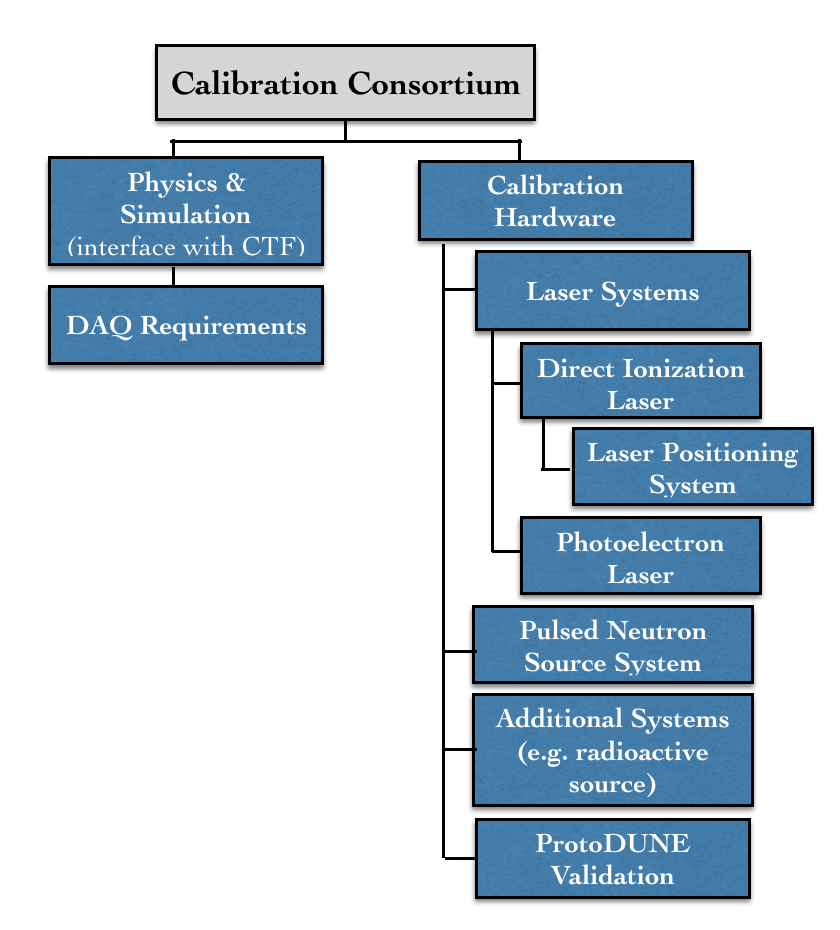
\includegraphics[height=4.0in]{graphics/calib_scope_chart.png}
%\caption{Calibration consortium subsystem chart.}
%\label{fig:scope_chart}
%\end{figure}

\begin{dunefigure}[Calibration consortium subsystem chart]{fig:calib_scope_chart}
{Calibration consortium subsystem chart.}
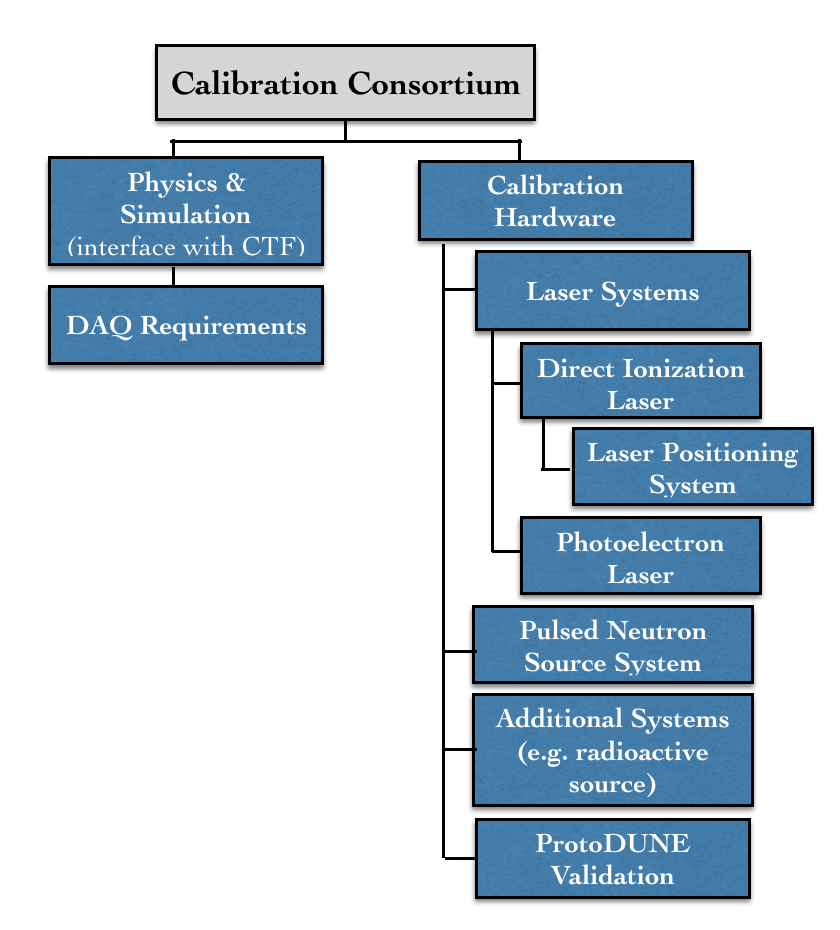
\includegraphics[height=4.0in]{graphics/calib_scope_chart.png}
\end{dunefigure}

%%%%%%%%%%%%%%%%%%%%%%%%%%%%
%\subsection{Requirements}
%\label{sec:sp-calib-ov-req}

%\input{vol-sp/ch-dp-calib-requirements}


%%%%%%%%%%%%%%%%%%%%%%%%%%%%
\subsection{Design Considerations and Requirements}
\label{sec:dp-calib-ov-consid}
%\fixme{SG, KM: Done; JM please check. }
%To-DO: Need more information on requirements from neutron source and RA source, once we have it, we can update the text/table as needed.}
%\fixme{SG/JM done; need to put in autogenerated requirements table; Anne et al., working on it}
Some common design considerations for calibration devices include stability, reliability, and longevity, so calibration systems can be operated for the lifetime of the experiment (\dunelifetime). Such longevity is uncommon for any device, so the overall design permits replacing devices where possible. The systems must also adhere to relevant global requirements of the \dword{dune} detector. Table~\ref{tab:specs:DP-CALIB} shows the top-level overall requirements for calibration subsystems. For example, \dword{dune} requires the \efield on any instrumentation devices inside the cryostat to be less than 30 kV/cm to minimize the risk of dielectric breakdown in \dword{lar}. Another consideration important for reconstructing events is the maximum noise level the readout electronics can tolerate from calibration devices. 
%\fixme{is the following sentence true for DP too? We need to either change it or remove it. SG: yes, PDDP is evaluating this.}
We are evaluating this using \dword{pddp}. 

Developing the \dword{sp} module calibration systems has already started, so the design considerations for \dword{dp} closely follow \dword{sp} while taking into account some important differences.

The longer drift length of \dpmaxdrift in \dword{dp} (instead of \spmaxdrift in \dword{sp}) suggests that diffusion causes a wider spread in the size of the electron cloud. For the nominal field of \dpnominaldriftfield, the transverse diffusion coefficient is \SI{13.1586}{\square \cm \per \s} \cite{Li:2015rqa,larpropertiesbnl}, leading
%% calculation sigma = sqrt(2*D_T*t) where t = L/v s the drift time
%% v = 0.1648 cm/us = 0.1648e6 cm/s
%% sqrt(2*13.1586*1200/(0.1648e6)) 
to a maximum spread of \SI{4.4}{\milli\m}; the maximum in \dword{sp}, for a \spmaxdrift drift, is \SI{2.4}{\milli\m}. Taking these values in quadrature with the readout pitch, which is smaller in \dword{dp}, the spatial precision is about \SI{5.3}{\milli\m}, comparable in both detectors. 

The longer drift length in \dword{dp} leads to proportionally higher ion charge accumulation and higher space charge effects. This is compounded by the fact that the charge multiplication in the gas phase leads to ion feedback into the liquid. We therefore expect larger \efield distortions in \dword{dp}, up to about \SI{15}{\%}~\cite{bib:boyu2018}.
%\fixme{JM: the next sentence, might be a bit too obvious, so I commented out to avoid a lengthy intro.}
However, the relative effect of a \SI{1}{\%} distortion of the \efield in the liquid phase on the amount of charge reaching the gas-liquid interface should be similar to the effect of a \SI{1}{\%} distortion of the \efield in the \dword{sp} on the amount of charge reaching the \dword{apa} wires. Therefore, in terms of energy response, the requirements on \efield measurement precision should be similar in both \dword{sp} and \dword{dp}.

%\paragraph{Laser system}
%{\bf Laser System:} 
For the laser system, the energy and position reconstruction requirements for physics measurements lead to requirements for precision in measuring the laser \efield as well as its spatial coverage and granularity. 
 The laser \efield measurement precision must be approximately \SI{1}{\%}, so the effect on the collected charge is well below \SI{1}{\%}. This is also motivated by consistency with the high level \dword{dune} specification of \SI{1}{\%} on field uniformity throughout the volume for component alignment and the \hv system. For laser coverage, to keep the overall \efield measurement at the $\sim$\SI{1}{\%} level, even with possible large distortions in the unmeasured region, the specification requires coverage of \SI{93}{\%} or more of the total \dword{fv}. This is more than in \dword{sp} because the maximum expected distortions are also larger. 
 The granularity requirement for the laser measurement is estimated based on the \dword{fv} uncertainty requirements (\SI{1}{\%}) and corresponding uncertainty requirements (\SI{1.5}{\cm}) in each coordinate. The required voxel size will depend on the magnitude of the \efield distortions. In regions of large distortions (of up to \SI{15}{\%}, which is possible because of gas phase ion feedback), \num{10}$\times$\num{10}$\times$\SI{10}{\cubic\cm} granularity is necessary, but  \num{30}$\times$\num{30}$\times$\SI{30}{\cubic\cm} should be sufficient for distortions up to \SI{5}{\%}, as discussed in Section~\ref{sec:dp-calib-laser-req}

The laser beam position must also meet the level of reconstruction requirement in each coordinate, approximately \SI{5}{\milli\m} over \SI{15}{\m}, where the latter is the distance between two consecutive laser ports in the beam direction. This results in a stringent requirement of \ang{0.03} (or \SI{0.5}{\mrad}). In terms of design constraints, the absence of detector elements (like \dwords{apa} and \dwords{cpa} in \dword{sp}) within the \dword{tpc} makes it easier to cover the \dword{dp} module with fewer beams, as long as \dword{fc} penetration is possible. 
%\fixme{JM: We already talk about this in the Interface section. Maybe we don't need to repeat here? I'm OK with commenting these next 2 sentences out. SG: agreed.}
%Interfaces with the \dword{pds} need careful evaluation, since it will not be possible to avoid hitting the reflector panels. The PMTs' HV will likely need to be turned off for the laser calibration. 

%The data volume for the ionization laser system must be at least \num{90}~TB/year/\SI{10}{\kt}, assuming \num{800}k laser pulses, \num{10}$\times$\num{10}$\times$\SI{10}{\cubic\cm} voxel sizes, a \SI{100}{\micro\s} zero suppression window, and one dedicated calibration campaign per year.\todo{Need to update DAQ calculation based on number of channels.}

The data volume for the ionization laser system must be at least \num{20}~TB/year/\SI{10}{\kt}, assuming \num{400}k laser pulses, \num{10}$\times$\num{10}$\times$\SI{10}{\cubic\cm} voxel sizes, a \SI{100}{\micro\s} zero suppression window, and one dedicated calibration campaign per year.

%\paragraph{\dlong{pns}}
%{\bf \dlong{pns}:} 
For the \dword{pns} system, fewer detector elements leads to a more uniform distribution of neutrons, an advantage of \dword{dp}. On the other hand, if injected from the top, the neutrons must penetrate the readout planes, which can reduce the neutron flux going into the argon. This is currently under investigation. For the \dword{pns} system, the system must provide a sufficient neutron event rate to make spatially separated precision measurements across the detector of a comparable size to the voxels probed by the laser (\num{30}$\times$\num{30}$\times$\SI{30}{\cubic\cm}) for most regions of the detector (\SI{75}{\%}). 
% 1st draft
%For the supernova program, measurements from the \dword{pns} \fixme{This abbreviation is in neither glossary.} should demonstrate 1\% energy scale, 5\% energy resolution, and 0.5 MeV detection threshold, so each voxel should have sufficient neutron event rate to achieve this. %\todo{KM: Improve or remind connection to SN program? even though it's comparable? SG: maybe for 2nd draft?}
%rewritten for 2nd draft
For the supernova program, the sensitivity to distortions of the neutrino energy spectrum depends on the uncertainties in the detection threshold and the reconstructed energy scale and resolution. Studies discussed in the physics \dword{tdr} \fixme{Does this require a LATEX location code?} present target ranges for the uncertainties in these parameters as a function of energy. The measurements with the \dword{pns} should provide response corrections and performance estimates, so those uncertainty targets are met throughout the whole volume, and so each voxel has a sufficient neutron event rate (percent level statistical uncertainty).

%\fixme{Insert correct reference to physics TDR ch7}
%\fixme{Put PNS in glossary and use that.}
In terms of data volume requirements, the \dword{pns} system needs approximately \num{100}~TB/year/\SI{10}{\kt}, assuming \num{e6} neutrons/pulse, \num{1000} neutron captures/\si{\cubic\m}
%m$^{3}$ 
and \num{1300} observed neutron captures per pulse, and six calibration runs per year.
%\todo{Need to update DAQ calculation based on number of channels.} 

Table~\ref{tab:fdgen-calib-all-reqs} shows the full set of requirements related to all calibration subsystems. More details on each requirement can be found under dedicated subsections.   
%\todo{SP-CALIB-3 is coming out weird in table 1.1, needs to be fixed.}

%\fixme{Can the second part of this title be put in a footnote to Table 1.1? SG: we would prefer to leave it here}

%\fixme{Anne uncommented 5/20 (uncomment when spec table available)}
%%% This file is generated, any edits may be lost.

\begin{longtable}{p{0.14\textwidth}p{0.13\textwidth}p{0.18\textwidth}p{0.22\textwidth}p{0.20\textwidth}}
\caption{Specifications for DP-CALIB \fixmehl{ref \texttt{tab:spec:DP-CALIB}}} \\
  \rowcolor{dunesky}
       Label & Description  & Specification \newline (Goal) & Rationale & Validation \\  \colhline

   
  \newtag{DP-CALIB-1}{ spec:efield-calib-precision }  & Ionization laser \efield measurement precision  &  \SI{1}{\%} &  \efield affects energy and position measurements. &  ProtoDUNE and external experiments. \\ \colhline
     % 1
   \newtag{DP-CALIB-2}{ spec:efield-calib-coverage }  & Ionization laser \efield measurement coverage  &  $>\,\SI{93}{\%}$ \newline ( \SI{100}{\%} ) &  Allowable size of the uncovered detector regions is set by the highest reasonably expected field distortions, \SI{15}{\%}. &  ProtoDUNE \\ \colhline
     % 2
   \newtag{DP-CALIB-3}{ spec:efield-calib-granularity }  & Ionization laser \efield measurement  granularity  &  \SI{10 x 10 x 10}{\centi\metre} \newline ( \SI{10 x 10 x 10}{\centi\metre} ) &  Minimum measurable region is set by the maximum expected distortion and position reconstruction requirements. &  ProtoDUNE \\ \colhline
     % 3
   \newtag{DP-CALIB-4}{ spec:laser-position-precision }  & Laser beam position precision  &  \SI{0.5}{\milli\radian} \newline ( $<\,\SI{0.5}{\milli\radian}$ ) &  The necessary spatial precision does not need to be smaller than the CRP strip spacing. &  ProtoDUNE \\ \colhline
     % 4
   \newtag{DP-CALIB-5}{ spec:neutron-source-coverage }  & Neutron source coverage  &  $>\,\SI{75}{\%}$ \newline ( \SI{100}{\%} ) &  Set by the energy resolution requirements at low energy. &  Simulations \\ \colhline
     % 5
   \newtag{DP-CALIB-6}{ spec:data-volume-laser }  & Ionization laser DAQ rate per year (per 10 kt)  &  $>\,\SI{20}{TB/yr/10 kt}$ \newline ($>\,\SI{40}{TB/yr/10 kt}$) &  The laser data volume must allow the needed coverage and granularity. &  ProtoDUNE and simulations \\ \colhline
     % 6
   \newtag{DP-CALIB-7}{ spec:data-volume-pns }  & Neutron source DAQ rate per year (per 10 kt)  &  $>\,\SI{100}{TB/yr/10 kt}$ \newline ( $>\,\SI{200}{TB/yr/10 kt}$ ) &  The pulsed neutron system must allow the needed coverage and granularity. &  Simulations \\ \colhline
     % 7


\label{tab:specs:just:DP-CALIB}
\end{longtable}
% This file is generated, any edits may be lost.
\begin{footnotesize}
%\begin{longtable}{p{0.14\textwidth}p{0.13\textwidth}p{0.18\textwidth}p{0.22\textwidth}p{0.20\textwidth}}
\begin{longtable}{p{0.12\textwidth}p{0.18\textwidth}p{0.17\textwidth}p{0.25\textwidth}p{0.16\textwidth}}
\caption{Specifications for DP-CALIB \fixmehl{ref \texttt{tab:spec:DP-CALIB}}} \\
  \rowcolor{dunesky}
       Label & Description  & Specification \newline (Goal) & Rationale & Validation \\  \colhline

   \newtag{DP-FD-1}{ spec:dp-min-drift-field }  & Minimum drift field  &  $>$\,\SI{250}{V/cm} \newline ( $>\,\SI{500}{V/cm}$ ) &  Lessens impacts of $e^-$-Ar recombination, $e^-$ lifetime, $e^-$ diffusion and space charge. &  ProtoDUNE \\ \colhline
    
   
  \newtag{DP-FD-2}{ spec:dp-system-noise }  & System noise  &  $<\,\SI{1000}\,e^-$ &  Studies suggest that a minimum of 5:1 S/N on individual strip measurements allows for sufficient reconstruction performance. &  ProtoDUNE and simulation \\ \colhline
    
   \newtag{DP-FD-5}{ spec:lar-purity }  & Liquid argon purity  &  $<$\,\SI{100}{ppt} \newline ($<\,\SI{30}{ppt}$) &  Provides $>$5:1 S/N on induction planes for  pattern recognition and two-track separation. &  Purity monitors and cosmic ray tracks \\ \colhline
    
   
  \newtag{DP-FD-7}{ spec:dp-misalignment-field-uniformity }  & Drift field uniformity due to component alignment  &  $<\,1\,$\% throughout volume &  Maintains TPC and  FC orientation and shape. &  ProtoDUNE \\ \colhline
    
   
  \newtag{DP-FD-9}{ spec:dp-crp-strip-spacing }  & CRP strips spacing  &  $<\,\SI{4.7}{mm}$ &  Enables 100\% efficient MIP detection, \SI{1.5}{cm} $yz$ vertex resolution. &  Simulation \\ \colhline
    
   
  \newtag{DP-FD-11}{ spec:dp-hvs-field-uniformity }  & Drift field uniformity due to HVS  &  $<\,\SI{1}{\%}$ throughout volume &  High reconstruction efficiency. &  ProtoDUNE and simulation \\ \colhline
    
   \newtag{DP-FD-13}{ spec:dp-fe-peak-time }  & Front-end peaking time  &  \SI{1}{\micro\second} \newline ( Adjustable so as to see saturation in less than \SI{10}{\%} of beam-produced events ) &  Vertex resolution &   \\ \colhline
    
   
  \newtag{DP-FD-22}{ spec:dp-data-rate-to-tape }  & Data rate to tape  &  $<\,\SI{30}{PB/year}$ &  Cost.  Bandwidth. &  ProtoDUNE \\ \colhline
    
   
  \newtag{DP-FD-23}{ spec:dp-sn-trigger }  & Supernova trigger  &  $>\,\SI{95}{\%}$ efficiency for a SNB producing at least 60 interactions with a neutrino energy >10 MeV in 12 kt of active detector mass during the first 10 seconds of the burst. &  $>\,$90\% efficiency for SNB within 100 kpc &  Simulation and bench tests \\ \colhline
    
   
  \newtag{DP-FD-24}{ spec:dp-local-e-fields }  & Local electric fields  &  $<\,\SI{30}{kV/cm}$ &  Maximize live time; maintain high S/N. &  ProtoDUNE \\ \colhline
    
   
  \newtag{DP-FD-25}{ spec:de-non-fe-noise }  & Non-FE noise contributions  &  $<<\,\SI{1000}\,e^- $ &  High S/N for high reconstruction efficiency. &  Engineering calculation and ProtoDUNE \\ \colhline
    
   
  \newtag{DP-FD-26}{ spec:dp-lar-impurity-contrib }  & LAr impurity contributions from components  &  $<<\,\SI{30}{ppt} $ &  Maintain HV operating range for high live time fraction. &  ProtoDUNE \\ \colhline
    
   
  \newtag{DP-FD-27}{ spec:dp-radiopurity }  & Introduced radioactivity  &  less than that from $^{39}$Ar &  Maintain low radiological backgrounds for SNB searches. &  ProtoDUNE and assays during construction \\ \colhline
    
   \newtag{DP-FD-29}{ spec:dp-det-uptime }  & Detector uptime  &  $>\,$98\% \newline ($>\,$99\%) &  Meet physics goals in timely fashion. &  ProtoDUNE \\ \colhline
    
   \newtag{DP-FD-30}{ spec:dp-det-mod-uptime }  & Individual detector module uptime  &  $>\,$90\% \newline ($>\,$95\%) &  Meet physics goals in timely fashion. &  ProtoDUNE \\ \colhline
    

   
  \newtag{DP-CALIB-1}{ spec:efield-calib-precision }  & Ionization laser \efield measurement precision  &  \SI{1}{\%} &  \efield affects energy and position measurements. &  ProtoDUNE and external experiments. \\ \colhline
    
   \newtag{DP-CALIB-2}{ spec:efield-calib-coverage }  & Ionization laser \efield measurement coverage  &  $>\,\SI{93}{\%}$ \newline ( \SI{100}{\%} ) &  Allowable size of the uncovered detector regions is set by the highest reasonably expected field distortions, \SI{15}{\%}. &  ProtoDUNE \\ \colhline
    
   \newtag{DP-CALIB-3}{ spec:efield-calib-granularity }  & Ionization laser \efield measurement  granularity  &  \SI{10 x 10 x 10}{\centi\metre} \newline ( \SI{10 x 10 x 10}{\centi\metre} ) &  Minimum measurable region is set by the maximum expected distortion and position reconstruction requirements. &  ProtoDUNE \\ \colhline
    
   \newtag{DP-CALIB-4}{ spec:laser-position-precision }  & Laser beam position precision  &  \SI{0.5}{\milli\radian} \newline ( $<\,\SI{0.5}{\milli\radian}$ ) &  The necessary spatial precision does not need to be smaller than the CRP strip spacing. &  ProtoDUNE \\ \colhline
    
   \newtag{DP-CALIB-5}{ spec:neutron-source-coverage }  & Neutron source coverage  &  $>\,\SI{75}{\%}$ \newline ( \SI{100}{\%} ) &  Set by the energy resolution requirements at low energy. &  Simulations \\ \colhline
    
   \newtag{DP-CALIB-6}{ spec:data-volume-laser }  & Ionization laser DAQ rate per year (per 10 kt)  &  $>\,\SI{20}{TB/yr/10 kt}$ \newline ($>\,\SI{40}{TB/yr/10 kt}$) &  The laser data volume must allow the needed coverage and granularity. &  ProtoDUNE and simulations \\ \colhline
    
   \newtag{DP-CALIB-7}{ spec:data-volume-pns }  & Neutron source DAQ rate per year (per 10 kt)  &  $>\,\SI{100}{TB/yr/10 kt}$ \newline ( $>\,\SI{200}{TB/yr/10 kt}$ ) &  The pulsed neutron system must allow the needed coverage and granularity. &  Simulations \\ \colhline
    


\label{tab:specs:DP-CALIB}
\end{longtable}
\end{footnotesize}

%Full requirements table (not autogenerated) is below for completeness.
\begin{dunetable}
[Full specifications for calibration subsystems]
{p{0.45\linewidth}p{0.25\linewidth}p{0.25\linewidth}}
{tab:fdgen-calib-all-reqs}
{Full list of Specifications for the Calibration Subsystems.}   
Quantity/Parameter	& Specification	& Goal		 \\ \toprowrule      

Noise from calibration devices	 & $\ll$ 1000 enc   & \\ \colhline    Max. \efield near calibration devices & < 30 kV/cm & <15 kV/cm \\ \colhline                     

\textbf{Direct Ionization Laser System} &    &   \\ \colhline   
\efield measurement precision & 1\% & <1\% \\ \colhline
\efield measurement coverage & > 93\% & 100\% \\ \colhline
\efield measurement granularity & < \num{10}$\times$\num{10}$\times$\SI{10}{\cubic\cm} & \num{10}x\num{10}x\num{10}~cm \\ \colhline
%Top field cage penetrations (alternative design) & to achieve desired laser coverage & \\ \colhline
DAQ rate per 10~kton & 20 TB/year & 40 TB/year \\ \colhline
Longevity	& \dunelifetime			& > \dunelifetime   \\ \colhline        
%Stability & Match precision requirement at all places/times	&  \\ \colhline  Reliability	& Measurements as needed & Measurements as needed \\ \colhline 
\textbf{Laser Positioning System} & & \\ \colhline                      
Laser beam position precision & 0.5~mrad & 0.5~mrad \\ \colhline
Longevity	& \dunelifetime			& > \dunelifetime   \\ \colhline        
%Stability & Match precision requirement at all places/times	&  \\ \colhline  Reliability	& Measurements as needed & Measurements as needed \\ \colhline    
\textbf{Photoelectron Laser System}	   &   &  \\ \colhline            
Longevity	& \dunelifetime			& > \dunelifetime   \\ \colhline        
%Stability & Match precision requirement at all places/times	&  \\ \colhline  Reliability	& Measurements as needed & Measurements as needed \\ \colhline

\textbf{Pulsed Neutron Source System}	   &   &  \\ \colhline        
Coverage & > 75\% & 100\% \\ \colhline
DAQ rate per 10~kton & 100~TB/year & 200~TB/year \\ \colhline 
Longevity	& 3 years			& \dunelifetime   \\ \colhline        
%Stability & Match precision requirement at all places/times	&  \\ 
%\colhline  Reliability	& Measurements as needed & Measurements as needed \\ \colhline

%\textbf{Proposed Radioactive Source System}	   &   &  \\ \colhline  
%Distance of the source from the field cage & 30 cm & \\ \colhline
%Rate of 9~MeV capture $\gamma$-events inside the source & < 1kHz & \\ \colhline 
%Data volume per 10~kton & 50~TB/year & 100~TB/year \\ \colhline 
%Longevity	& \dunelifetime			& > \dunelifetime   \\ \colhline    
%Stability & Match precision requirement at all places/times	&  \\ \colhline  Reliability	& Measurements as needed & Measurements as needed \\ \colhline

\end{dunetable}

%\fixme{ Where shall we put the following text?\\
%For the RSDS, ports will need to be selected close to the end-walls. An advantage of this system in DP is that the source movement is along the drift direction, so several runs can be taken at different positions along the drift coordinate, which is important to check the detector response.
%}

\subsection{Cryostat Configuration for Calibration}
\label{sec:calib-ports}
Figure~\ref{fig:DPFDLaserPositions} shows a possible layout of the laser calibration port locations on the cryostat roof. The penetrations dedicated for laser calibrations are shown in black circles. 
%The ports on far east and far west are outside the \dword{fc}. The current plan is to use these penetrations for several different purposes. For example, the penetrations on the far east and west will be used both by laser and radioactive source systems (if deployed). In addition to these dedicated ports, the \dword{dss} and cryogenic ports (orange and blue dots in Figure~\ref{fig:FTmap}) will also be used as needed to route cables for calibration systems (e.g., the \dword{sp} \dword{pds}). \dword{dss} and cryogenic ports can be accommodated with feedthroughs with a CF63 side flange for this purpose.   

%\begin{figure}[tbp]
%\centering
%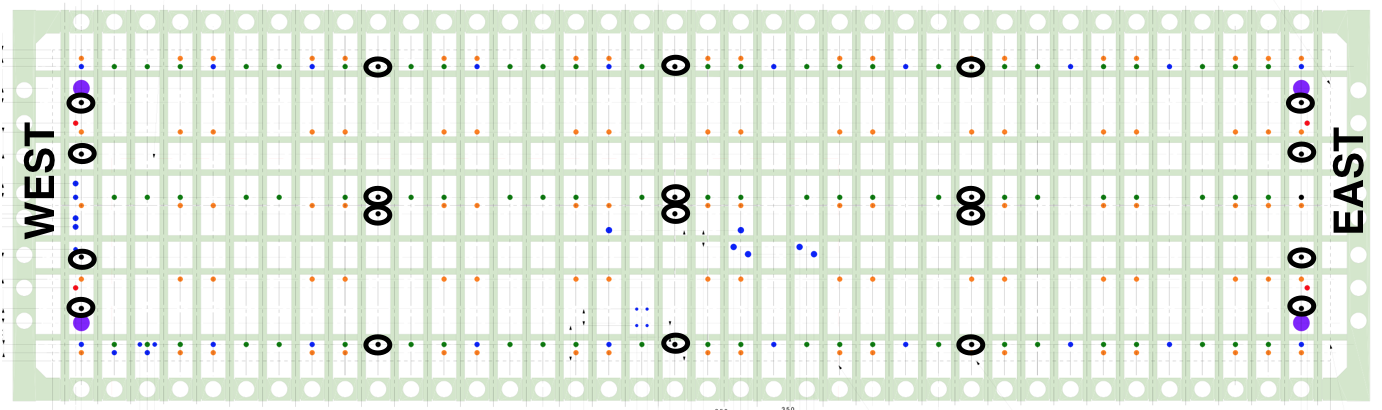
\includegraphics[height=2.0in]{FTmap.png}
%\caption{Top view of the \spmod %DUNE SP FD 
%cryostat showing various penetrations. Circles highlighted in black are multi-purpose calibration penetrations. The green dots are \dword{tpc} signal cable penetrations. The blue ports are cryogenic ports. The orange ports are \dword{dss} penetrations. The larger purple ports at the four corners of the cryostat are human access ports.}
%\label{fig:ftmap}
%\end{figure}

\begin{dunefigure}[Sketch of cryostat penetration map with laser calibration ports]{fig:DPFDLaserPositions}
{Top view of the \dpmod %DUNE SP FD 
cryostat showing possible laser system penetrations (black circles). The red line shows the \dword{fc} top view and the green square is one of the six \dword{crp} modules. 
%Circles highlighted in black are multi-purpose calibration penetrations. The green dots are \dword{tpc} signal cable penetrations. The blue ports are cryogenic ports. The orange ports are \dword{dss} penetrations. The larger purple ports at the four corners of the cryostat are human access ports.
}
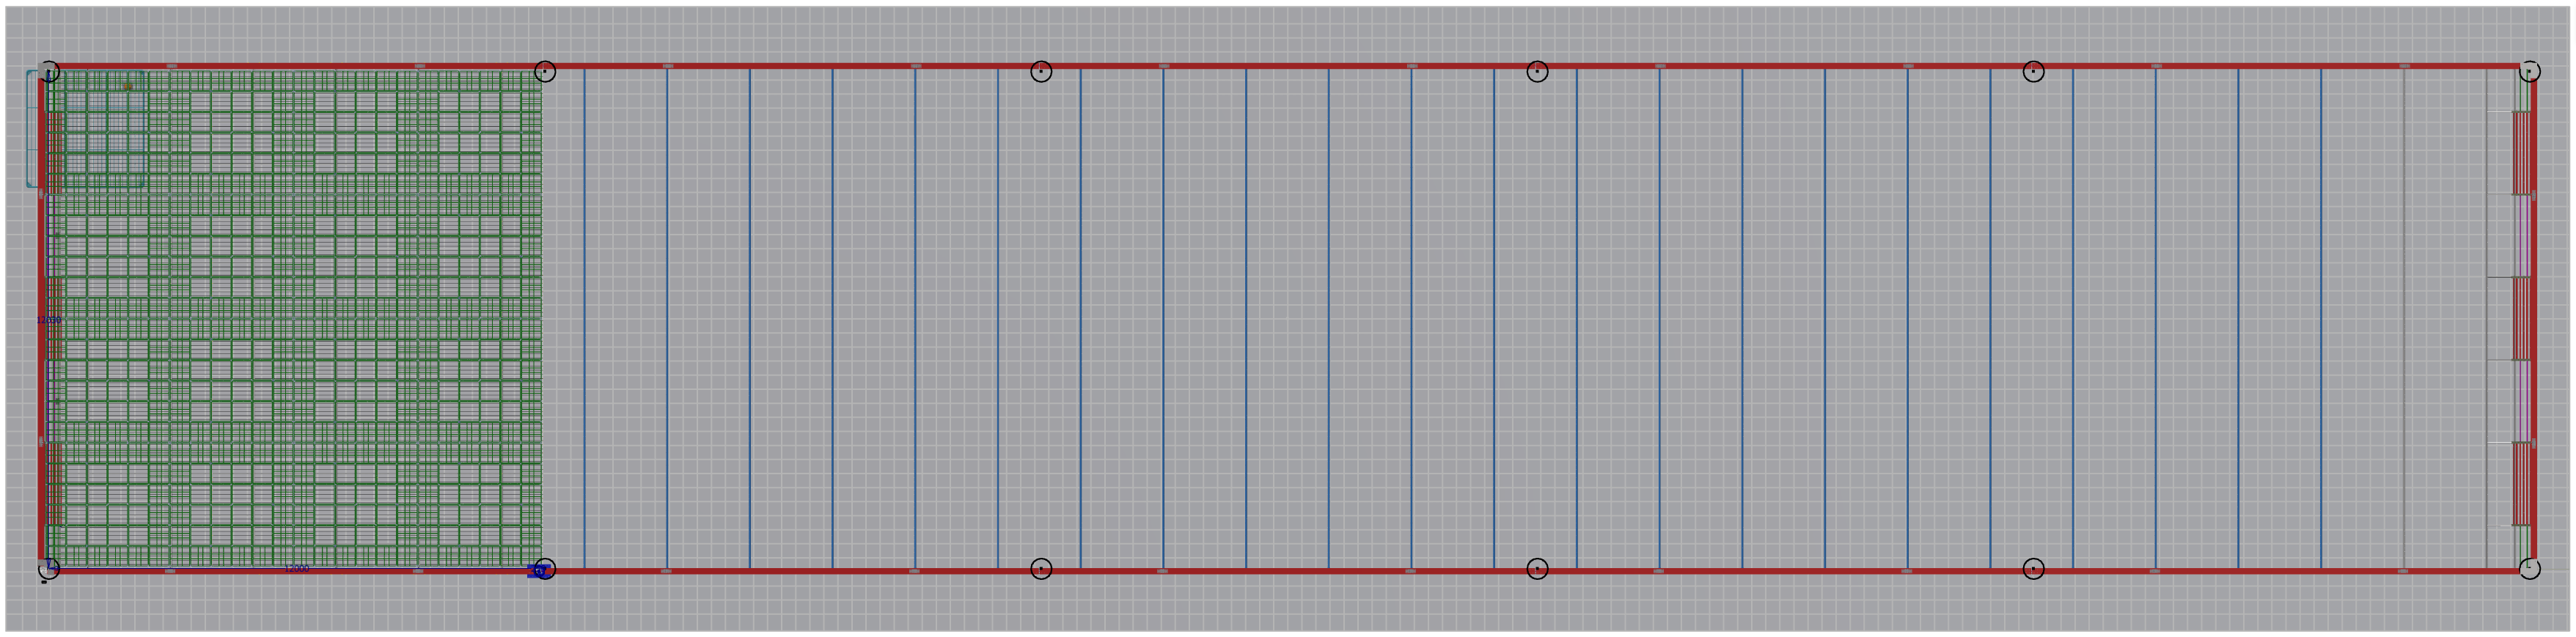
\includegraphics[width=1.0\textwidth]{DPFDLaserPositions.png}
\end{dunefigure}


The placement of these penetrations is driven by requirements of the ionization laser system and the available gaps between \dword{crp} and \dword{fc}.
%and radioactive source system. 
%The ports that are %inwards 
%towards the center of the cryostat are placed near the \dwords{apa} to minimize any risks due to the \dword{hv} discharge. For the far east and west ports, \dword{hv} is not an issue as they are located outside the \dword{fc} and the penetrations are located near mid-drift (location favorable to possible source deployment).
%to meet radioactive source requirements. 
%\fixme{The amendment above may need some work. I won't look at it until it's ready.}
Implementing the ionization laser system as proposed in Section~\ref{sec:dp-calib-sys-las-ion} requires \num{12} feedthroughs at each of the indicated ports. 
%the four \dword{tpc} drift volumes; this arrangement allows lasers to be used for full volume calibration of the E field and associated diagnostics (e.g., \dword{hv}). 

The distance between any two consecutive feedthrough columns in Figure~\ref{fig:DPFDLaserPositions} should be approximately \SI{12}{\m}, which is reasonable because experience from the \dword{microboone} laser system shows that tracks will propagate over that detector's full \SI{10}{\m} length. Assuming that the effects of Rayleigh scattering and self-focusing (Kerr effect) do not limit the laser track length, this laser arrangement could illuminate the full volume with crossing track data.  Please note that, at this time, the maximum usable track length is unknown, and the full \SI{60}{\m} \detmodule  length may be covered by the laser system after optimization.

%The exact location of the \dword{pns} ports is not yet finalized, but two ports, each at 1/4 of the module length (along beam direction) from each side should be close to optimal. 

For the \dword{pns} system, two ports, each at 1/4 of the module length (along the beam direction) from each side should be close to optimal to provide necessary coverage.

For the proposed \dword{rsds} system, ports must be close to the end-walls. An advantage of this system in \dword{dp} is that the source movement is along the drift direction, so several runs can be taken at different positions along the drift coordinate, which is important to check the detector response.

Between \num{4} and \num{10} additional ports should be available for the \dword{pns} system (toward middle of the cryostat) and the proposed \dword{rsds} system (close to the east and west end-walls). The exact locations of these additional ports is not yet finalized.

%\end{comment}
